\newpage
\subsection{Sicherungsbereiche}
Die Sicherung wird in Bewegung immer über die Uhrzeit ausgegeben. Sowohl in Fahrzeugen als zu Fuß in Marschformationen.  Die Marschrichtung ist immer 12 Uhr. \\
\subsubsection{Rundumsicherung}
Die Rundumsicherung bedeutet, dass 360° von dem Trupp abgesichert werden, jeder Soldat hat dazu den Auftrag, ein Viertel des „Kreises“ abzusichern. Jeder Feind in diesem Viertel ist die Verantwortung des Soldaten. Rundumsicherung kann aus dem Marsch und in einer Stellung vollzogen werden. In Stellung geht es nicht darum, einen perfekten Kreis zu bilden – sondern sich in Deckung zu bewegen und von dort aus seinen Sektor zu sichern. Je nach Bedarf kann der Truppführer sich, um z.B. zu funken, eine 4 Mann Sicherung aufbauen lassen. \\
Standardsicherung  – 4 Team: 
\begin{itemize}
\item Nr.1 sichert auf 12 Uhr 
\item Nr.2 sichert auf 9 Uhr 
\item Nr.3 sichert auf 3 Uhr 
\item Nr.4 sichert auf 6 Uhr 
\end{itemize}
\begin{figure}[htbp]
	\centering
	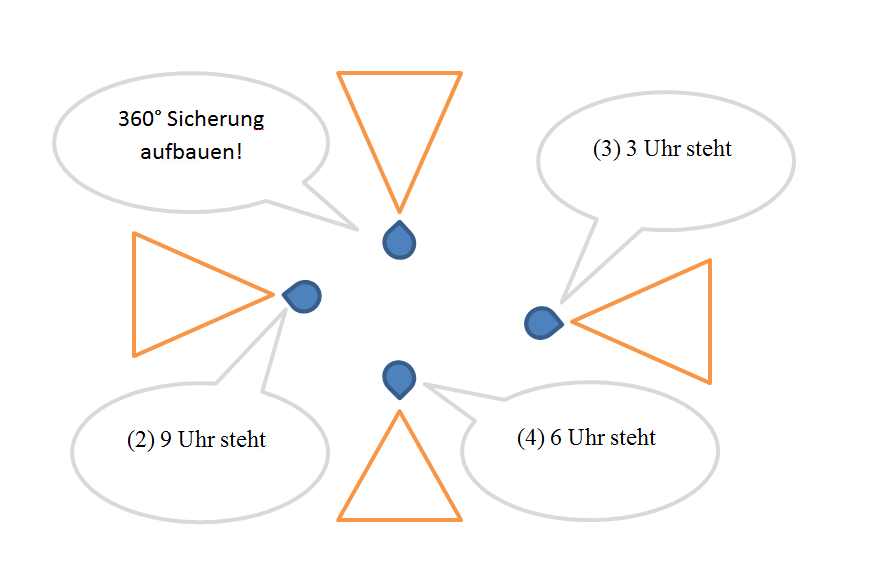
\includegraphics[width=15cm]{./Grafiken/Abschnitt/360er.png}
	\caption{4 Mann 360er}
\end{figure}
Standardsicherung – 6 Team: 
\begin{itemize}
\item Nr.1 sichert auf 12 Uhr 
\item Nr.2 sichert auf 9 Uhr 
\item Nr.3 sichert auf 3 Uhr 
\item Nr.6 sichert auf 6 Uhr
\item Nr.4 und Nr.5 springen ein bzw. unterstützen Schwerpunkte. Nr.1 kann die Verantwortung für die 12 Uhr beispielsweise an die Nr.2 abgeben – in der Stellung kann das MG auf einen Schwerpunkt verlegt werden (aus der ein Feind erwartet wird). 
\end{itemize}
\begin{figure}[htbp]
	\centering
	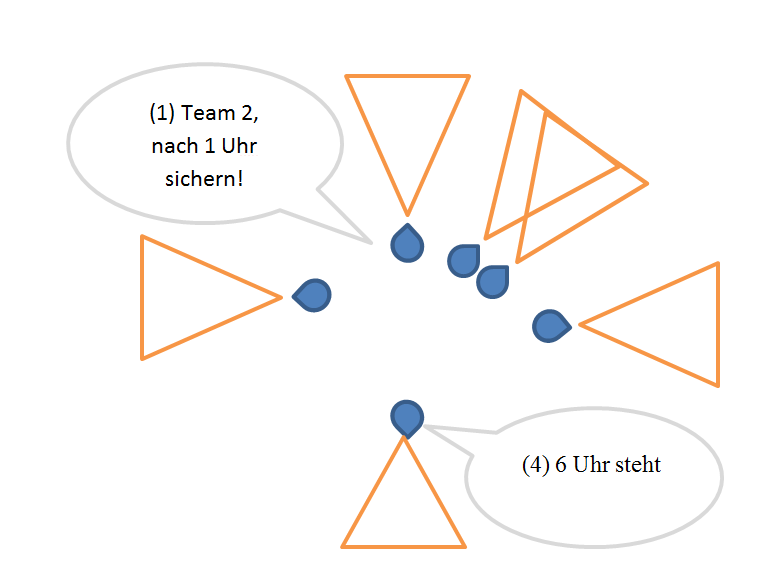
\includegraphics[width=15cm]{./Grafiken/Abschnitt/360erFS.png}
	\caption{6 Mann 360er mit Feuerschwerpunkt}
\end{figure}
\begin{figure}[htbp]
	\centering
	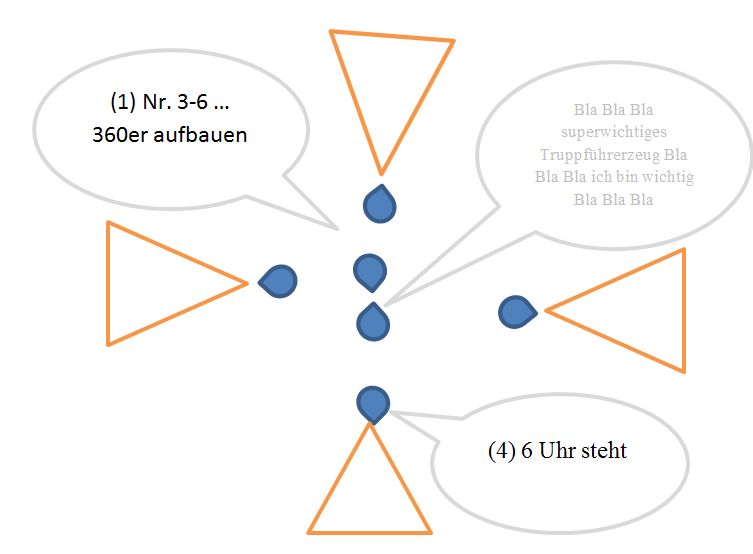
\includegraphics[width=15cm]{./Grafiken/Abschnitt/360erOTF.png}
	\caption{6 Mann 360er entlastetes Führungsteam}
\end{figure}
\subsubsection{180°-Sicherung}
Die 180-Grad-Sicherung ist eine Halbkreis-Sicherung. Wird in der Regel an Mauern angewandt – oder in einer Stellung, um ein zu beobachtendes Gelände abzusichern, wenn der Rückraum als absolut sicher gilt. Zu beachten ist, dass die 180° Sicherung nicht unmittelbar an der Mauer sondern etwa 1m entfernt aufgebaut wird. So können einzelne Soldaten oder Trupps hinter der Sicherung kreuzen, ohne in den eigenen Feuerbereich treten zu müssen. \\
\begin{figure}[htbp]
	\centering
	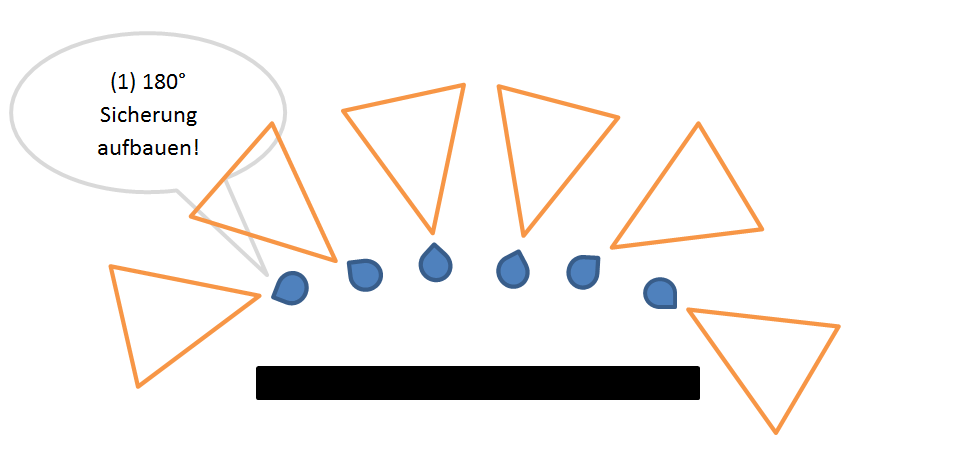
\includegraphics[width=15cm]{./Grafiken/Abschnitt/180er.png}
	\caption{180° Sicherung an Mauer}
\end{figure}
\subsection{Fahrzeuge}
\subsubsection{Auf- und Ab sitzen}
Fahrzeuge werden in umgekehrte Trupp Reihenfolge betreten. (Siehe auch „Richtig Funken und Kommunizieren im Trupp“) \\
\subsubsection{Sicherungsbereich}
Der Sicherungsbereich nach Verlassen des Fahrzeuges entspricht den Standsicherungsbereichen für  Trupps (siehe Kolonne \autoref{Kolonne}, Standartsicherung 360°). Mehrere Trupps können sich z.B. 180° Sicherungsbereiche abstimmen. \\
Kommando Verlassen:  Alle Truppteile verlassen das Fahrzeug \\
Kommando Absitzen: Schütze bleibt, Fahrer bleibt in Nähe am Fahrzeug, Rest baut Sicherung auf.  \\
Wichtig:
\begin{itemize}
\item Bewegungskorridor vor und hinter dem Fahrzeug immer frei lassen. 12 Uhr ist immer die Fahrzeugfront.
\item Ein Fahrzeug in ARMA ist keine Deckung, wenn der Gegner AT-Waffenbesitzt.
\item Abstand halten:  Wenn nicht anders befohlen, 20 Meter Abstand vom Fahrzeug. Fahrzeuge tendieren zum Explodieren, bieten schlechte Deckung  und brauchen zudem jederzeit Platz für Manöver.
\end{itemize}
\begin{figure}[htbp]
	\centering
	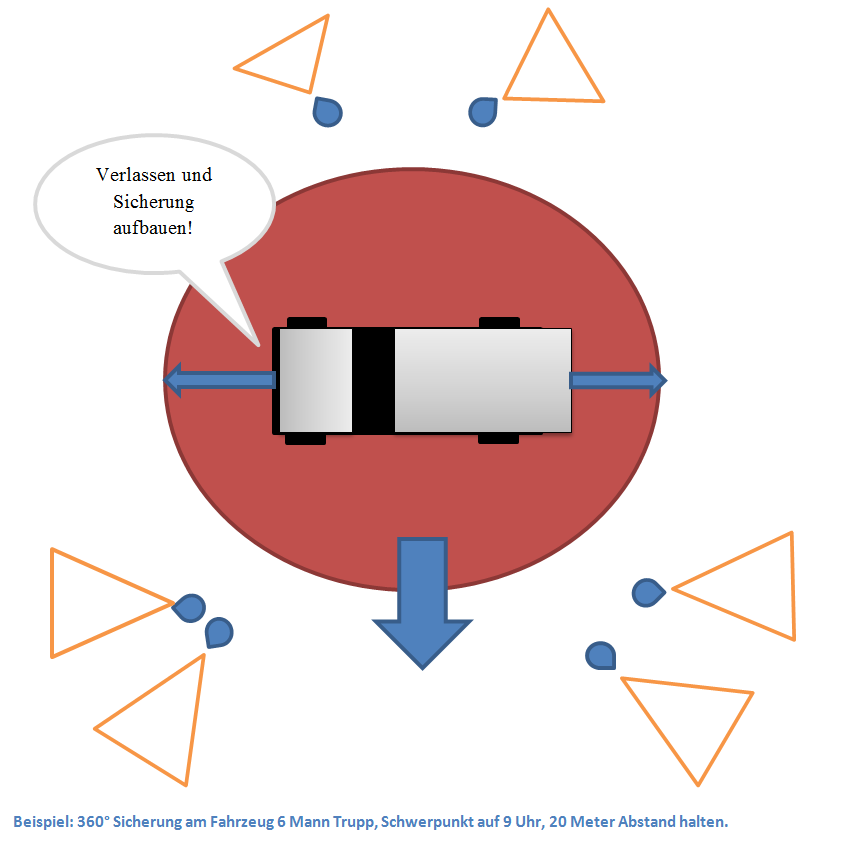
\includegraphics[width=15cm]{./Grafiken/Abschnitt/Fahrzeug_verlassen.png}
	\caption{Absitzen und Sicherung beim Fahrzeug}
\end{figure}
